\documentclass{article}
\usepackage[margin=1in]{geometry}
\usepackage{amsmath,amsthm,amssymb}
\usepackage{bbm,enumerate,mathtools}
\usepackage{tikz,pgfplots}
\usepackage{chessboard}
\usepackage[hidelinks]{hyperref}
\usepackage{multicol} % Problem 35
\usepackage{xstring} % Difficulty command
\usetikzlibrary{shapes.geometric}

\newenvironment{question}{\begin{trivlist}\item[\textbf{Question.}]}{\end{trivlist}}
\newenvironment{note}{\begin{trivlist}\item[\textbf{Note.}]}{\end{trivlist}}
\newenvironment{references}{\begin{trivlist}\item[\textbf{References.}]}{\end{trivlist}}
\newenvironment{related}{\begin{trivlist}\item[\textbf{Related.}]\end{trivlist}\begin{enumerate}}{\end{enumerate}}

\newcommand\score[1]{
\pgfmathsetmacro\pgfxa{#1+1}
\tikzstyle{scorestars}=[
  star,
  star points=5,
  star point ratio=2.25,
  draw,
  inner sep=3pt,
  anchor=outer point 5
]
  \begin{tikzpicture}[baseline]
    \draw[opacity=0] (0,-0.5) rectangle (0,0.2); % Workaround for whitespace at the bottom.
    \foreach \i in {1,...,4} {
      \pgfmathparse{(\i<=#1?"yellow":"gray")}
      \edef\starcolor{\pgfmathresult}
      \draw (\i*4.5ex,0) node[name=star\i,scorestars,fill=\starcolor]  {};
    }
  \end{tikzpicture}
}

\newcommand{\difficulty}[1]{%
  \IfEqCase{#1}{%
      {1}{
        
\begin{tikzpicture}[scale=0.7, baseline=0.9mm]%
          \definecolor{slopegreen}{rgb}{0.0, 0.5, 0.0}%
          \fill[slopegreen] (0.5,0.5) circle (0.5);%
        \end{tikzpicture}%
      }%
      {2}{
        
\begin{tikzpicture}[scale=0.7, baseline=0.9mm]%
          \definecolor{slopeblue}{rgb}{0.0, 0.44, 1.00}
          \fill[slopeblue] (0,0) rectangle (1,1);%
        \end{tikzpicture}%
      }%
      {3}{
\begin{tikzpicture}[scale=0.7, baseline=0.9mm]\fill (0,0.5)--(0.5, 0)--(1,0.5)--(0.5,1)--cycle; \end{tikzpicture}}%
      {4}{
\begin{tikzpicture}[scale=0.7, baseline=0.9mm]\fill (0.25,0)--(0,0.5)--(0.25,1)--(0.5,0.5)--cycle; \fill (0.75,0)--(0.5,0.5)--(0.75,1)--(1,0.5)--cycle;\end{tikzpicture}}%
      % you can add more cases here as desired
  }[\PackageError{difficulty}{Undefined difficulty level: #1}{}]%
}%
\newcommand{\rating}[2]{\difficulty{#1}\\\score{#2}\\}


\begin{document}
  Start with $n$ piles with a single stone in each pile. If two piles have the
  same number of stones, then any number of stones can be moved between them.
\begin{figure}[!h]
  \centering
  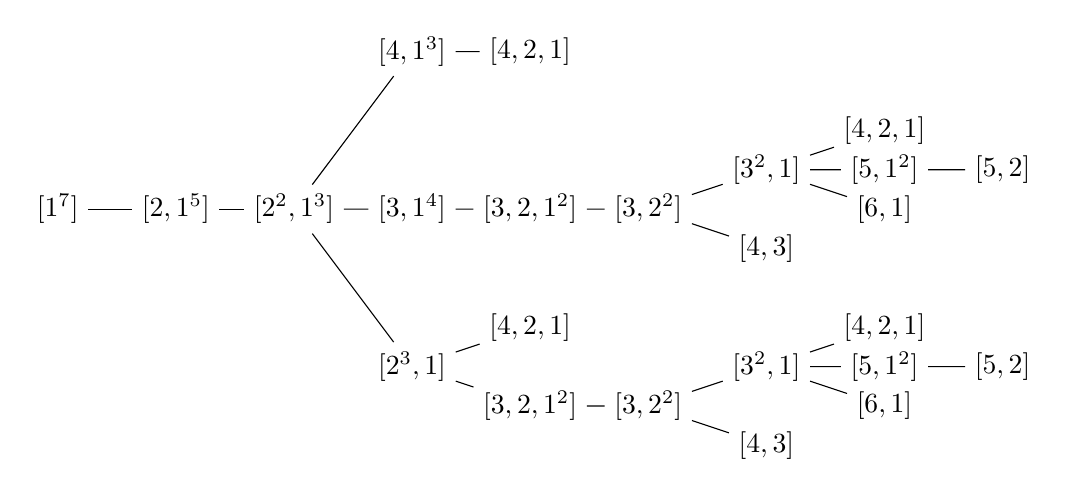
\begin{tikzpicture}[
    level distance=1.5cm,
    level 3/.style={sibling distance=2cm},
    level 4/.style={sibling distance=1cm},
    level 6/.style={sibling distance=1cm},
    level 7/.style={sibling distance=0.5cm},
    grow'=right
  ]
    \node {$[1^7]$}
      child[grow=right] { node {$[2, 1^5]$}
        child { node {$[2^2, 1^3]$}
          child { node {$[2^3, 1]$}
            child { node {$[3, 2, 1^2]$}
              child { node {$[3, 2^2]$}
                child { node {$[4, 3]$} }
                child { node {$[3^2, 1]$}
                  child { node {$[6, 1]$}}
                  child { node {$[5, 1^2]$}
                    child { node {$[5, 2]$}}
                  }
                  child { node {$[4, 2, 1]$}}
                }
              }
            }
            child { node {$[4, 2, 1]$} }
          }
          child { node {$[3, 1^4]$}
            child { node {$[3, 2, 1^2]$}
              child { node {$[3, 2^2]$}
                child { node {$[4, 3]$} }
                child { node {$[3^2, 1]$}
                  child { node {$[6, 1]$} }
                  child { node {$[5, 1^2]$}
                    child { node {$[5, 2]$} }
                  }
                  child { node {$[4, 2, 1]$} }
                }
              }
            }
          }
          child { node {$[4, 1^3]$}
            child { node {$[4, 2, 1]$}}
          }
        }
      };
  \end{tikzpicture}
  \caption{
    An illustration of all possible moves for $n = 7$.
  }
\end{figure}

\begin{question}
  What is the greatest number of steps that can occur? Alternatively how many
  ``levels'' are in the tree of possible moves?
\end{question}

\begin{related}
  \item Let $A292726$ be the total number of distinct states. What is $A292726$?
    (e.g. $A292726(7) = 14$.)
  \item Let $c = A000041 - A292726$ be the total number of states that \textit{cannot} be acheived.
    (e.g. $c(5) = 1$ via the state $[5]$.)
  \item Is $c(p) = 1$ for all primes $p$? Is $c(n) = 0$ if and only if $n$ is a power of $2$?
  \item Let $\ell = A292836$ be the least number of steps to a terminal state.
    (e.g. $\ell(7) = 4$ ending in $[4,2,1]$.)
  \item Let $g = A292729$ be the greatest number of steps to a terminal state.
    (e.g. $g(7) = 8$ ending in $[5,2]$.)
  \item Let $p$ be the total number of paths, i.e. the number of leaves in the
    tree. (e.g. $p(7) = 10$.)
  \item Let $t$ be the number of distinct \textit{terminal} states.
    (e.g, $t(7) = 4$ via $[4,2,1]$, $[4,2]$, $[6, 1]$, and $[4, 3]$.)
  \item What if you can move stones between any sets of piles that share the
    same number of stones? (e.g. $[2^3] \rightarrow [6]$ or $[2^3] \rightarrow [4, 1, 1]$)
\end{related}

\begin{references}
  \item \url{https://oeis.org/A292836}
\end{references}
\end{document}
